\chapter{Related Work}\label{2_relatedWork}
%This section presents related work to a slacklining assistance system with an interactive technology approach. It provides exercises and feedback for beginners on a slackline with the Microsoft Kinect v2 as a tracking device. Hence it is necessary to have a good overview about existing systems, approaches and studies that can help to build an appropriate concept and system. First related concepts regarding slacklining show how to build learning techniques for beginners, the efficacy of it in balance training, and areas of application. Next current tracking technologies have to be compared for tracking the human body on the slackline and why the Microsoft Kinect v2 seems like the appropriate tracking device. Lastly the system has to be aware of cognitive load and motivating aspects, which can be challenging with repetitive exercises. Several applications show where problems occur with different feedback and interaction methods. Also design opportunities for guiding the user through the learning process are demonstrated by various approaches.

This section presents related work to a slacklining assistance system with an interactive technology approach. It provides exercises and feedback for beginners on a slackline with the Microsoft Kinect v2 as a tracking device. Hence it is necessary to provide instructive teaching methods for beginners. Therefore, existing approaches and studies have been elaborated to build an appropriate foundation and point out several application scenarios. Also the user interface should motivate the slacker for the training scenario and lead to a proper user experience.

First related concepts regarding slacklining show how to build learning techniques for beginners, the efficacy of it in balance training, and areas of application. Next current tracking technologies have to be compared for tracking the human body on the slackline and why the Microsoft Kinect v2 seems like the appropriate tracking device. The system has also be aware of the cognitive load and motivating aspects, which can be challenging with repetitive exercises. Several applications show where problems occur with different feedback and interaction methods. Lastly design opportunities for guiding the user through the learning process are demonstrated by various approaches.

\section{Slackline Specific Training and Effects to the Human Body}\label{2_2_slacklineTraining}

%The slacklining assistance system should mainly train and support beginners, or so called slackers, to walk on the slackline. Beyond that new skill acquisition for further training should be appropriately realised with the system. Therefore it is important to have a concrete baseline about what exercises and tips are useful for very beginners. Prior research justifies the applicability for areas like sport medicine and rehabilitation training in which such a system could be embedded. It could be used as an alternative to classical balance training because the slackline itself varies largely in space and the user has to use the whole body to balance her swift on the line~\cite{Pfusterschmied2013-yy}. Donath et al.~\cite{Donath2016-rt} found in his meta-analysis significant improvements in the postural control after slackline training, which indicates the efficacy of this training method on the human body.
As in other sport activities it is important to have a concrete baseline about which exercises and tips are useful for early beginners.
Mainly to have a good knowledge of the basics, which results in a faster learning process, but also to prevent injuries from the beginning.
In the following, several slackline learning techniques will be discussed, which are then be implemented in the SLS afterwards.
Prior research indicates the applicability of slackline training for areas like sport medicine and rehabilitation training.
It shows why slacklining could be used as an alternative to classical balance training and how the body swift affect these.
Donath et al.~\cite{Donath2016-rt} found in his meta-analysis significant improvements in the postural control after slackline training, which indicates the efficacy of this sport.
This subsection shows several application scenarios in which a slackline can be implemented and improve the training effect.

\subsection{Exercises During Slackline Training}\label{2_1_1_slacklineTraining}

For beginners it is often difficult to walk or even stay on a slackline. The uncontrollable swift of the narrow line result in unfamiliar movements that cannot be handled at the very beginning. Therefore they should learn to concentrate, build up motoric basics and trust into the line, as well as manage their body behaviour.

Thoman~\cite{Thomann2013-aa} differentiates two basic methods for the learning process on a slackline.
First, teaching a slacker without any external help or second, with systematic external assistance.
The investigation of Kroiß~\cite{Kroiss2007-ab} resulted in no significant difference between both methods.
However, there is a trend regarding providing methodological aid, like human support or physical objects as nordic walking sticks or a bar, can help to improve the learning effect (see Figure \ref{fig:supportiveExercises}).
Therefore, it is a good advise for beginners to learn the fundamentals of standing and walking on the slackline to build up a groundwork.
Several basic techniques and tips are useful to support her in this way.
For example focusing on a specific point in front of her, stretching out the arm, raising the hands over the shoulder level, turning the palms to the top, going slightly in the knees, having the feet straight with the line, and so on~\cite{Kleindl2011-bl, Kroiss2007-ab}.

\begin{figure}[htb]
	\centering
	\begin{minipage}[t]{0.23\linewidth}
		\centering
		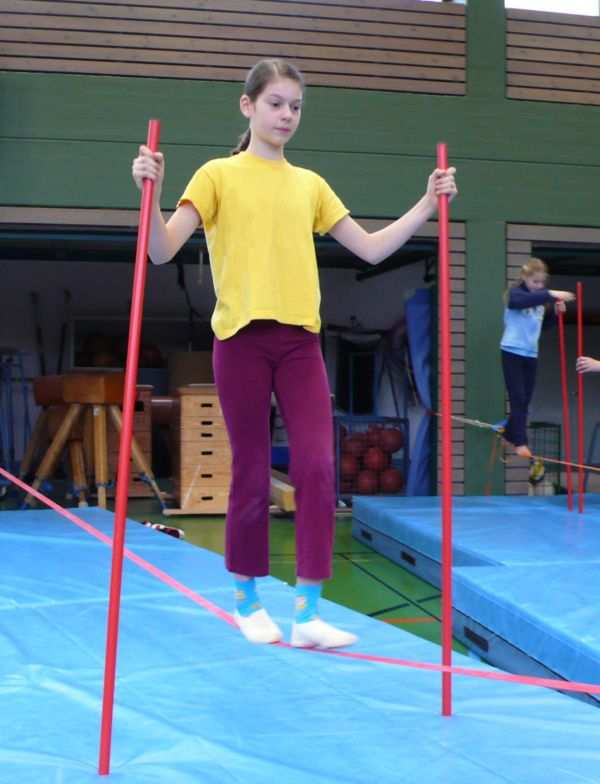
\includegraphics[width=1\linewidth]{Pictures/slacklineHelpSticks}
		\subcaption{Stick support}
		\label{fig:slacklineHelpSticks}
	\end{minipage}
	\hfill
	\begin{minipage}[t]{0.37\linewidth}
		\centering
		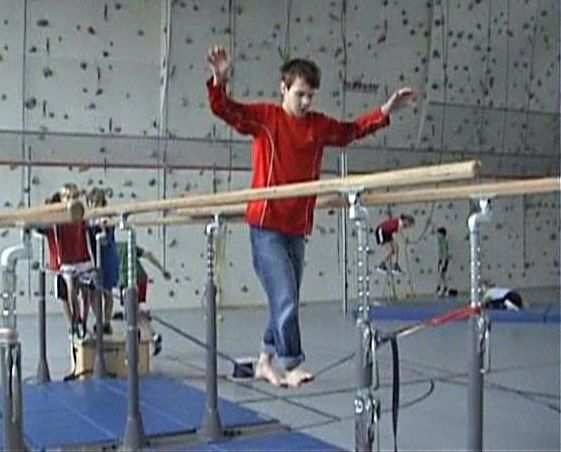
\includegraphics[width=1\linewidth]{Pictures/slacklineHelpBar}
		\subcaption{Between bars}
		\label{fig:slacklineHelpBar}
	\end{minipage}
	\hfill
	\begin{minipage}[t]{0.3\linewidth}
		\centering
		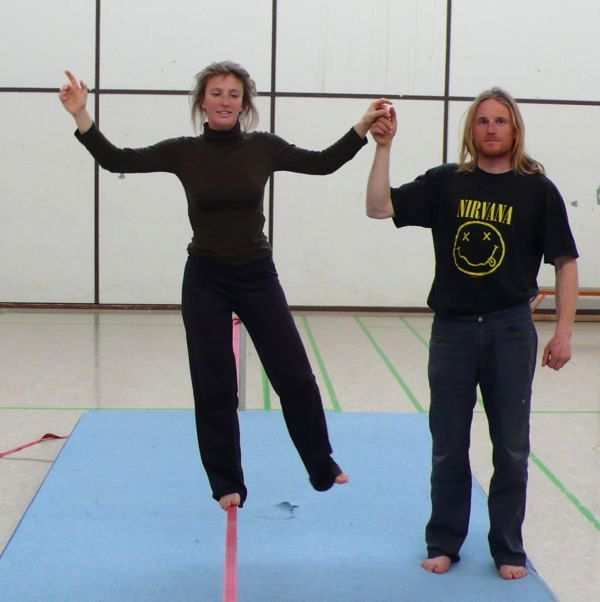
\includegraphics[width=1\linewidth]{Pictures/slacklineHelpHuman}
		\subcaption{Human support}
		\label{fig:slacklineHelpHuman}
	\end{minipage}
	\caption{Supportive exercises~\cite{Kroiss2007-ab}}
	\label{fig:supportiveExercises}
\end{figure}

With further progress, the external help, if given, should be reduced. The slacker can now try to stay and walk on the line on her own. It is recommended to begin with the practice of a basic start, to stay with both feet, and one feet on the slackline since these are basic techniques (see Figure \ref{fig:basicExercises}). Staying with both feet seems easier in the beginning but only the hips and hands can be used for balancing. With just one feet on the line, the slacker can use the other one as an additional extremity for balancing purposes.
%For this one feet stays on the line and the other nearby on the ground. With a little swing the bodie's center of gravity should be brought over the slackline. A fundamental technique is to stay on one and both feet.

\begin{figure}[htb]
	\centering
	\begin{minipage}[t]{0.30\linewidth}
		\centering
		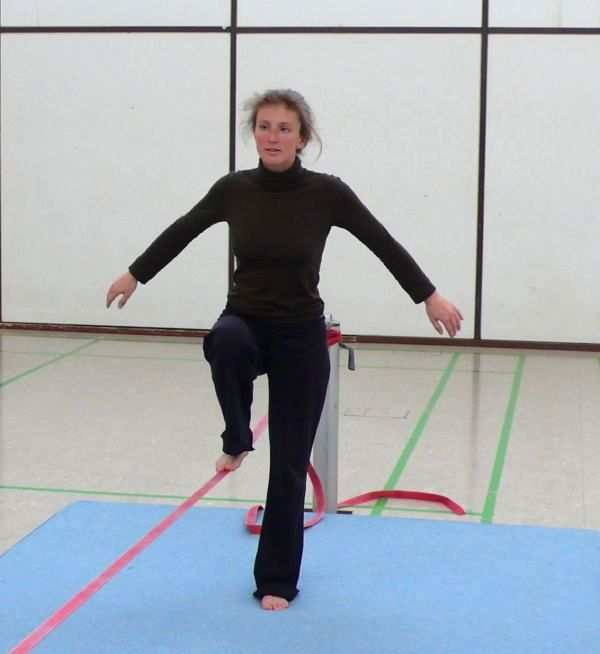
\includegraphics[width=1\linewidth]{Pictures/slacklineBasicStart}
		\subcaption{Basic start}
		\label{fig:slacklineBasicStart}
	\end{minipage}
	\hfill
	\begin{minipage}[t]{0.20\linewidth}
		\centering
		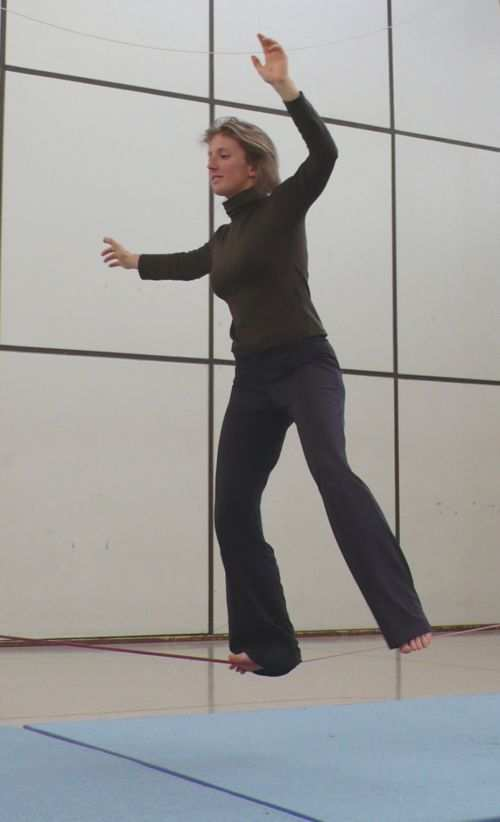
\includegraphics[width=1\linewidth]{Pictures/slacklineBasicOneFeet}
		\subcaption{One feet}
		\label{fig:slacklineBasicOneFeet}
	\end{minipage}
	\hfill
	\begin{minipage}[t]{0.33\linewidth}
		\centering
		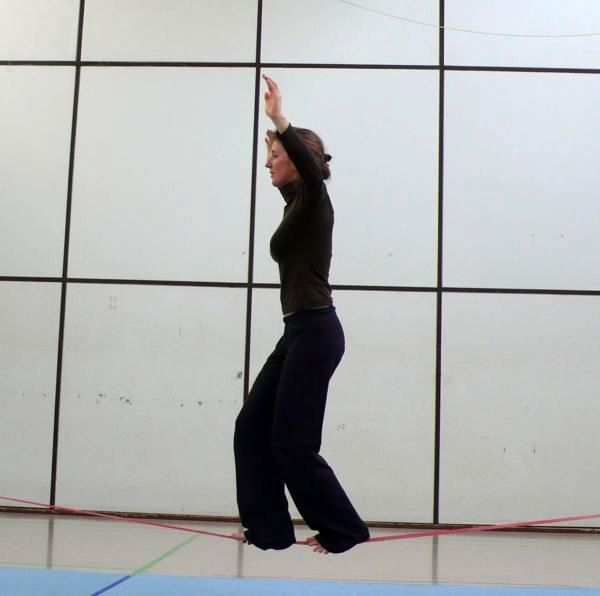
\includegraphics[width=1\linewidth]{Pictures/slacklineBasicBothFeet}
		\subcaption{Both feet}
		\label{fig:slacklineBasicBothFeet}
	\end{minipage}
	\caption{Basic exercises~\cite{Kroiss2007-ab}}
	\label{fig:basicExercises}
\end{figure}

Advanced training should be practiced in a more dynamical way~\cite{Thomann2013-aa}. Like seen in several research works~\cite{Donath2013-kk, Donath2016-gm, Granacher2010-ow, Keller2012-xh, Pfusterschmied2013-yy} this can be from crossover start (see Figure \ref{fig:slacklineAdvancedCrossoverStart}), turning on the line, hands on hips or behind the back (see Figure \ref{fig:slacklineAdvancedHandsBehindBack}), walk sidewards or backwards up to catch and pass a pall, kicking a football, bouncing a basketball, or a kneel down on the slackline (see Figure \ref{fig:slacklineAdvancedDropknee}).

\begin{figure}[htb]
	\centering
	\begin{minipage}[t]{0.28\linewidth}
		\centering
		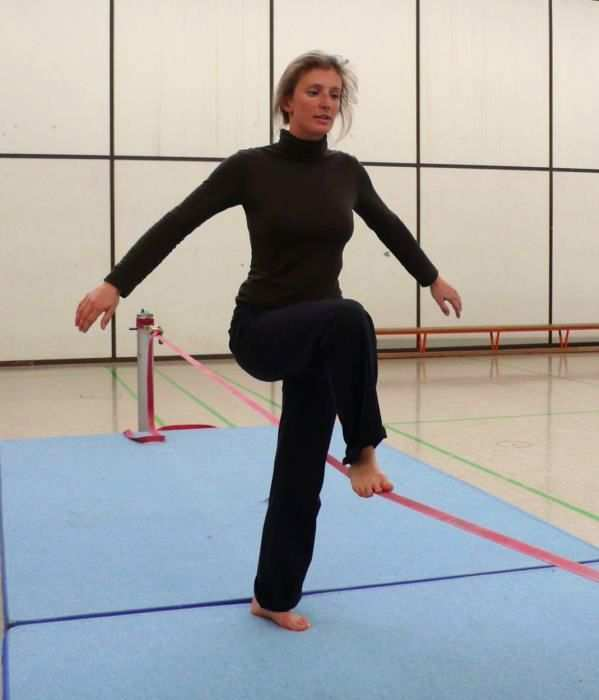
\includegraphics[width=1\linewidth]{Pictures/slacklineAdvancedCrossoverStart}
		\subcaption{Crossover start}
		\label{fig:slacklineAdvancedCrossoverStart}
	\end{minipage}	
	\hfill
	\begin{minipage}[t]{0.3\linewidth}
		\centering
		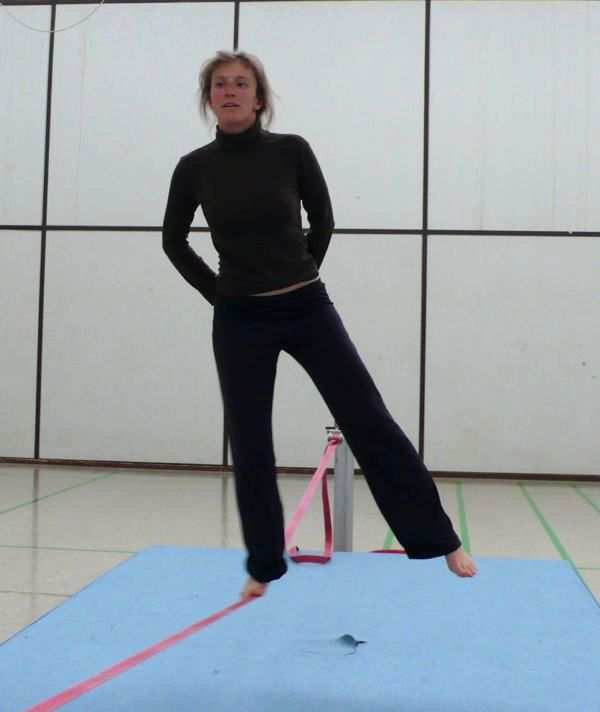
\includegraphics[width=0.9\linewidth]{Pictures/slacklineAdvancedHandsBehindBack}
		\subcaption{Hands behind back}
		\label{fig:slacklineAdvancedHandsBehindBack}
	\end{minipage}	
	\hfill
	\begin{minipage}[t]{0.38\linewidth}
		\centering
		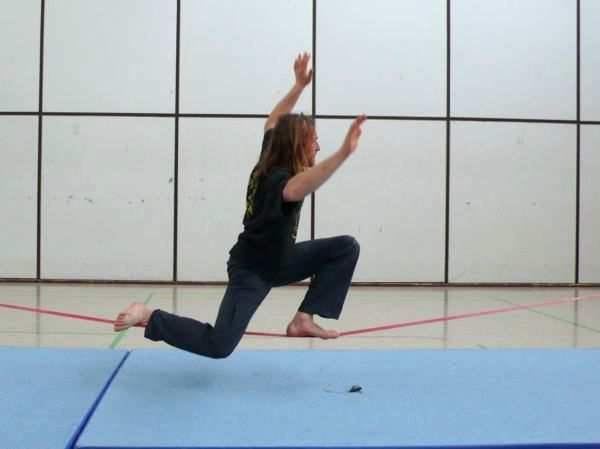
\includegraphics[width=1\linewidth]{Pictures/slacklineAdvancedDropknee}
		\subcaption{Dropknee}
		\label{fig:slacklineAdvancedDropknee}
	\end{minipage}	
	\caption{Advanced techniques~\cite{Kroiss2007-ab}}
	\label{fig:advancedExercises}
\end{figure}

Additional cognitive load is caused by unfamiliar exercises and simultaneous balancing on the line. This conjunction can lead to impairments. Even more difficult exercises can be carried out in further sessions like standing up from a sitting position, juggling, two people on the same line, reading a newspaper, closing eyes while balancing, vertical jumps, or rope skipping. Due to the higher difficulty of constraints, it results in a more unstable movement of the line.

Changes directly on the slackline itself, like varying the tension and length, have also an influence on the stability of the human body on the line~\cite{Keller2012-xh, Pfusterschmied2013-yy, Pfusterschmied2013-kq}. A short and tight line results in a relatively small vibrating area, where the slacker has to outbalance short unpredictable movements on point. Given a longer and loose line, it results in a more swinging behaviour that she has to counteract~\cite{Kroiss2007-ab}.
 
The slacklining assistance system should mainly train and support beginners to walk on the slackline.
With those approaches in mind, a foundation is set to build helpful exercises for the system.
Because the focus relies especially on beginners, this information serves as a guideline for supporting them with effective and efficient methods.
Now is the question, what effect has slacklining on the human body and in which application areas can it be applied?
This is part of the next subsection.

\subsection{Slackline Specific Training Effects and Application Scenarios}

Donath et al.~\cite{Donath2013-kk} elaborated the effects of slackline training on regular balancing, jump performance, and muscle activity with young children in school sport. The slackline specific balance has improved. Also the dynamic sway and muscle activity for the lower limb is reduced. However, there were no effects regarding jump performance. The children enjoyed the slackline training. In comparison to classical balance training, it can be more fun for the children and at the same time serve as an effective training method.

A further study of Donath et al.~\cite{Donath2016-gm} investigated slackline training with seniors from an age between 59 to 69 to measure effects on slackline specific balance and neuromuscular performance. They found significant differences between pre- and posttests during all slackline stance conditions. In addition the trunk and limb muscle activity were reduced after the training phase. With this in mind slacklining can be provided as an alternative balance training method for seniors. Regular balance training can help to reduce the fall risk, which can be an useful therapy for seniors when keeping in mind that 30\% of seniors suffer from fall injuries once a year.

Keller et al.~\cite{Keller2012-xh} examined the improvement of the postural control regarding the Hoffmann-Reflex after slackline training and whether adaptations can be found regarding classical balance training. The H-Reflex (Hoffmann-Reflex) is used to assess and quantify stretch-reflex responses due to electrical stimulation. The measurements show that these were significantly reduced as well as slackline specific balance were improved. Therefore slackline training and classical balance training have at least similar effects on the postural control.

Pfusterschmied et al.~\cite{Pfusterschmied2013-yy} found significant effects regarding stable stance after slackline training and even more effects were found for perturbed leg stance. This is because slacklining is a high dynamic movement activity and there is more need of regaining equilibrium as in perturbed stance than for maintaining balance as in a stable leg stance condition. The velocity in medio-lateral and anterior-posterior center of gravity, knee and hip joint is reduced as well as the range motion in knee and hip joint. No changes in medio lateral direction for the stable surface or joint kinematics for both have been found.

Another study of Pfusterschmied et al.~\cite{Pfusterschmied2013-kq} shows effects on lower limb joint motion and muscle activation. They found a decrease in platform velocity and improvements in corrective action in the knee joint. Also enhanced activation of the muscle activity in rectus femoris (upper leg) was measured.

Granacher et al.~\cite{Granacher2010-ow} investigated the impact of slackline training for balance and strength promotion and found contradictory results compared with the studies described above. Static and dynamic postural control were analysed as well as the isometric and dynamic muscle strength. There were no effects regarding the postural control, maximal torque, and jumping height. The results can be explained due to the assessment of other recorded variables, usage of different methods for analysing the data, and the relatively short slackline training time than in other studies~\cite{Pfusterschmied2013-yy}. Therefore this study can be seen as an exceptional case.

Those investigations show that slacklining is indeed an effective method for improving the postural control. Hence many application scenarios can be thought of to implement a slacklining assistance system. For example it can be used as a training approach in school sport, preventative activity for seniors, and rehabilitation alternative. Furthermore it can be used as a supportive training method for athletes in sport activities like skiing or skating, that require a good body balance. Interactive technologies can be used to support training in such scenarios. The next section provides an overview about state of the art technologies, compares them, and show several implementations in balance scenarios.\label{2_1_slacklineTraining}

\section{Interactive Technology}\label{2_3_interactiveTechnology}

To build a real time feedback assistance system, a tracking device is needed that supports the slacker in an appropriate way and that won't interrupt her.
The Microsoft Kinect v2 seems like a suitable tracking system in this context, because the user doesn't need any further devices to be tracked as it will be discussed in the following.
%But it should be compared with other tracking technologies like the Nintendo Wii, Playstation Move, and motion capture systems to justify its usage.
Further, advantages and drawbacks of comparable systems like the Nintendo Wii, Playstation Move, and motion capture systems will be discussed.
Lastly, several studies show how accurate and precise the Microsoft Kinect v2 is, if it can be applied for balancing purposes, and if it gives the user appropriate feedback or useful analysis data for specialists like therapists.

\subsection{Comparison of Tracking Technologies} \label{trackingTechnologie}

The Nintendo Wii consists of a sensor bar with infrared sensors that estimates the position of the Wiimote controller in 3D. Further an accelerometer is integrated in the Wiimote to detect its motion. Thus the user can interact with the console, based on predefined gestures~\cite{Bogdanovych2015-ci, Tanaka2012-ACO}. Gesture recognition is an essential aspect of the slacklining assistance system for giving appropriate feedback regarding the executed exercise. Schlömer et al.~\cite{Schlomer2008-uo} analysed the gesture recognition of the Wii and found an error rate between 5\% and 15\%.

A similar approach with a handheld controller is followed by the PlayStation Move. It consists of a RGB camera called Move Eye that is used for tracking the 3D position of a glowing sphere attached on the handheld device named Move wand. The controller contains an accelerometer, gyro sensor and geomagnetic sensor to track the rotation. Further it  also supports position tracking. In this way more accurate tracking is possible than with the Nintendo Wii~\cite{Bogdanovych2015-ci, Tanaka2012-ACO}.

Both systems are suitable devices if the controller itself can be replicated as a virtual device like for example in golf or tennis. However, they do not track the body movement and the user is bound to her handheld devices to interact with the system. In the slacklining system they could disturb user standing on the slackline. Moreover accurate feedback from the whole body is wanted and thus it should be the actual controlling device. Therefore they seem not to be appropriate devices for the slacklining system.

With a motion capture suit, like \textit{Xsens MVN}~\cite{XsensMvn} or \textit{OptiTrack}~\cite{OptiTrack}, sensors or markers have to be attached on the user’s body for tracking her body motion and rotational data. This makes it the best method for high accuracy and precision body tracking. Problems with the suite are that it is very expensive and the setup takes relatively long time because of the marker attachment and the positioning of the tracking cameras. The biggest drawback is the uncomfortable bulky equipment that could interfere the user during the performance~\cite{Bogdanovych2015-ci, Chang2012-hz, Nusman2006-rf}. This makes it an inappropriate device for user tracking on a slackline.

The Microsoft Kinect is a static device that includes a RGB camera and depth sensor. Because the body joints and player position are recognised by these, the user is free in her movement without any further controller. Another advantage is the low price in comparison to the motion control suite, and the low setup time because only the device itself is needed. Problems occur with occlusion of body parts that results in glitches and flawed tracking~\cite{Kajastila2014-ug, Tang2015-wt}. To the user they can be hidden, e.g. by only showing the output of the depth cam~\cite{Holsti2013-kn}. This problem can also occur in the slacklining case because the feet overlay with each other while walking on the line. Therefore a technical feasibility evaluation have been conducted to show if this is a bigger problem or can be neglected.
%Therefore a feasibility study should be realised to show if this is a bigger problem or can be neglected. 
%The results can be seen in section \textbf{<NUMBER>}. 

With this in mind, the Microsoft Kinect v2 seems like the most suitable device. The recognition of the whole body, freedom of movement, short setup time, and relatively low cost make it the best system out of the considered systems.

\subsection{Accuracy of the Microsoft Kinect}

In the field of balance training it is necessary to give appropriate feedback for the patient that reveals errors in the performance and support a proper execution. With this in mind user tracking should be good enough to fulfil this criteria. Since Microsoft Kinect is used as the tracking device the accuracy and precision should be assessed.

Lim et al.~\cite{Lim2015-pw} assessed the accuracy of the Kinect with a 3D motion capture system as a reference system. For further understanding please review Figure \ref{fig:bodyWikiAnatomicalTermsOfLocation} regarding expressions to body planes and anatomical directional references. The participants had to execute balance training with complex aperiodic movements in the body planes (see Figure \ref{fig:bodyPlanes}). Similar characterization of movements are provided by the Kinect in comparison to the 3D motion capture system. The correlation analysis showed that the Kinect and the 3D motion capture system are highly correlated for the flexion and extensions in the medio-lateral-axis (x-axis) but not on the anterior-posterior-axis (y-axis) and the cranial-caudal-axis (z-axis) (see Figure \ref{fig:bodyDirectionalReferences}). This is because the Kinect determine joint locations based on the depth image data and the data input is limited to the depth camera view. Therefore recognition of joint angles in the sagittal and transverse plane is not optimal (see Figure \ref{fig:bodyPlanes}). Also the primary goal of the Kinect is to measure the dynamic movements in the coronal (frontal) plane for gaming reasons. It is indeed an effective system to characterize changes in center of mass and movements in the frontal plane during balance training. But it would not be suitable in balance training that require in-depth analyses of joint motions, which is not needed with the slackline assistance.

\begin{figure}[htb]
	\centering
	\begin{minipage}[t]{0.38\linewidth}
		\centering
		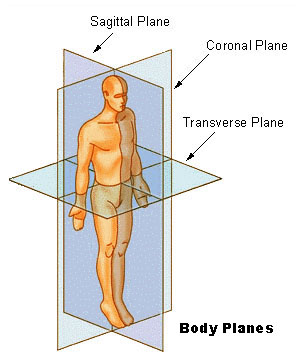
\includegraphics[width=1\linewidth]{Pictures/bodyPlanes}
		\subcaption{Picture of the planes of human anatomy~\cite{Wiki2017-bopl}}
		\label{fig:bodyPlanes}
	\end{minipage}
	\hfill
	\begin{minipage}[t]{0.6\linewidth}
		\centering
		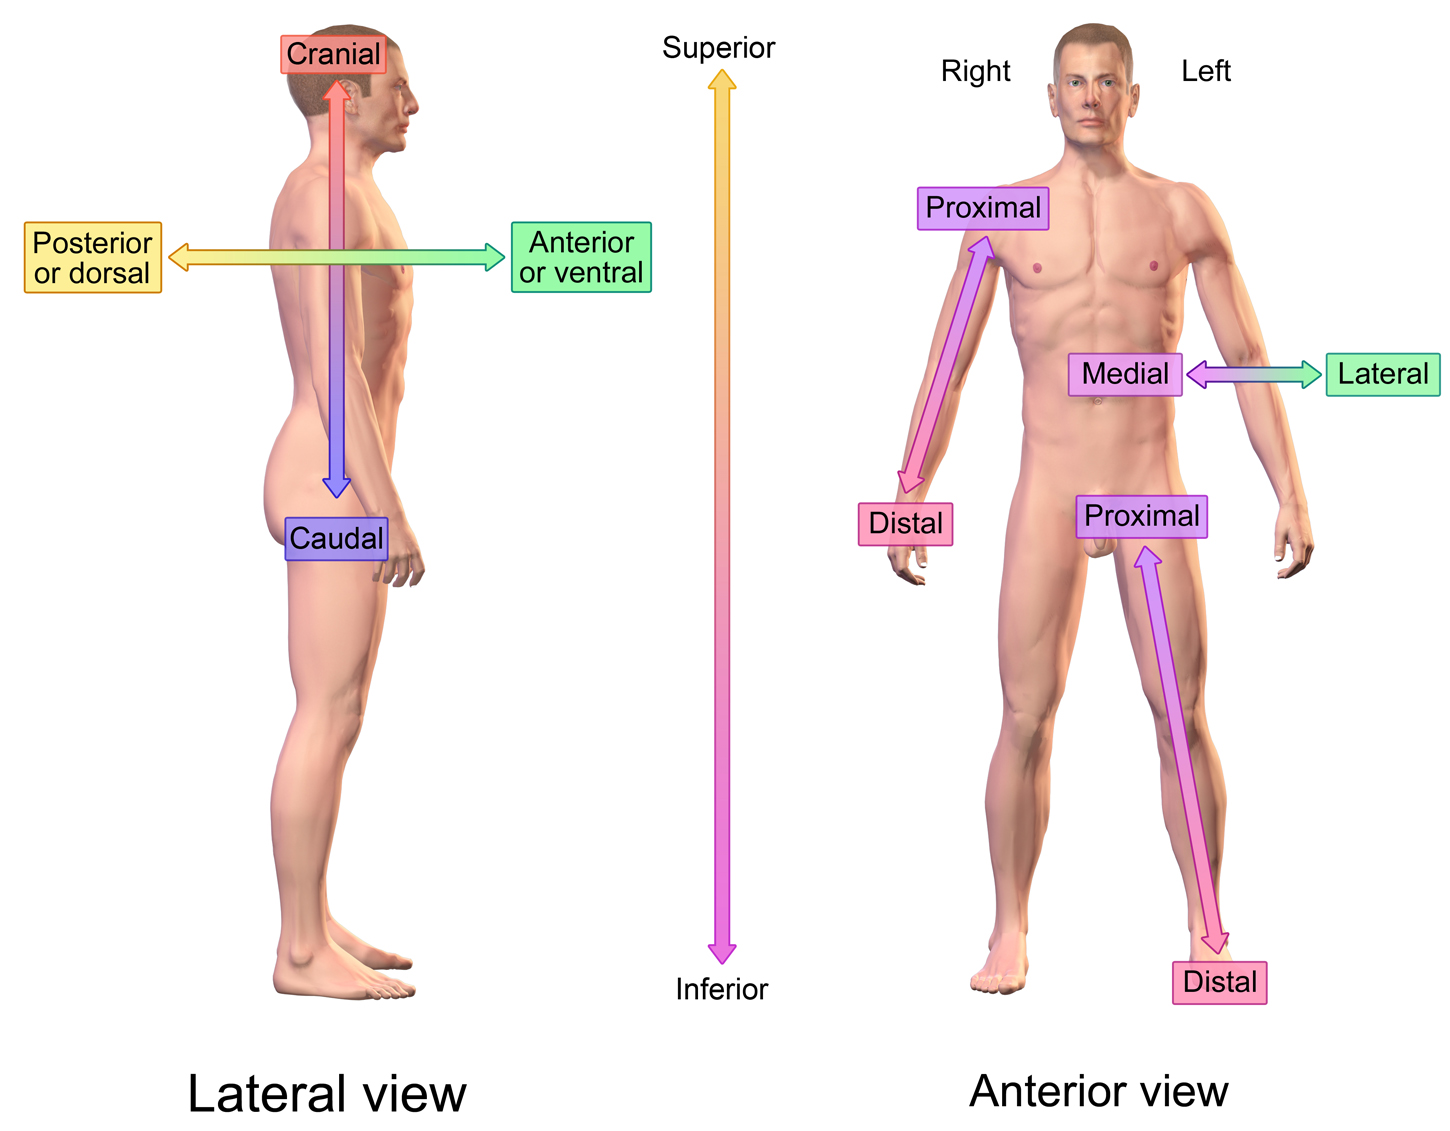
\includegraphics[width=1\linewidth]{Pictures/bodyDirectionalReferences}
		\subcaption{Anatomical directional references of the human body~\cite{Wiki2017-atol}}
		\label{fig:bodyDirectionalReferences}
	\end{minipage}
	\caption{Anatomical terms of location}
	\label{fig:bodyWikiAnatomicalTermsOfLocation}
\end{figure}

Chang et al.~\cite{Chang2012-hz} focuses mainly on the tracking performance of the Microsoft Kinect as a rehabilitation device in comparison with a high fidelity motion capture system called OptiTrack. In their application the user has to move objects from one side of the screen to the other. Five correct and incorrect movements have been realised and both systems successfully identified them. In trajectory comparison the results of the hand and elbow by the Kinect are very close to the OptiTrack system. Tracking of the shoulder movements are moderate because it involves rotation that the device does not recognizes well. The timing performance comparison shows that the OptiTrack system is negligible faster than the Kinect.

Woolford~\cite{Woolford2015-ub} compared the accuracy and precision of the Kinect v2 with the Qualisys motion capture system for the usage in healthcare applications. He describes that accuracy is the amount of how close a measured quantity to the actual value is. Precision is the similarity of repeated measurements (see Figure \ref{fig:systemAccuracyAndPrecisiong}). For example the Kinect skeleton tracking methods are accurate because the average joint position data is very close to the actual physical position. Regarding his definition of precision, the joint position data is not always precise because the data spreads in its position of the frame. The results show that the Kinect V2 is accurate but imprecise for body parts whose center of mass cannot be easily identified like the shoulder. For smaller body parts as well as between two body parts such as elbow or wrist the accuracy and precision is very high. 

\begin{figure}[htb]
	\centering
	\begin{minipage}[t]{0.49\linewidth}
		\centering
		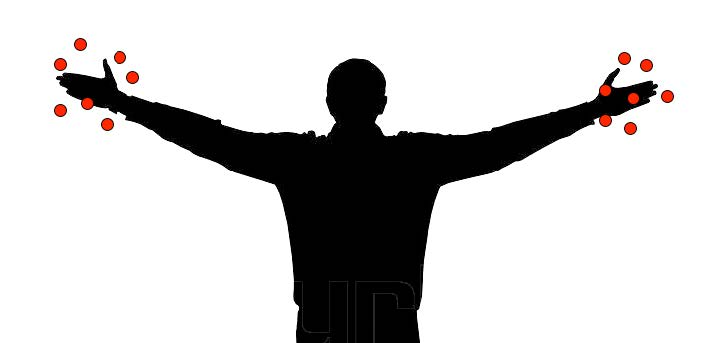
\includegraphics[width=1\linewidth]{Pictures/systemInaccurateImprecise}
		\subcaption{Inaccurate and imprecise system generates random-like measurements}
		\label{fig:systemInaccurateImprecise}
	\end{minipage}
	\hfill
	\begin{minipage}[t]{0.49\linewidth}
		\centering
		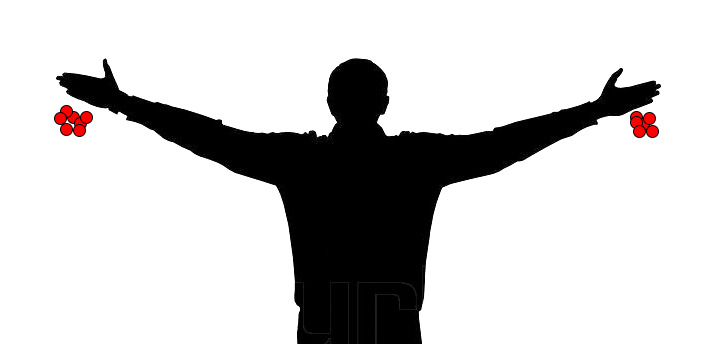
\includegraphics[width=1\linewidth]{Pictures/systemInaccuratePrecise}
		\subcaption{Inaccurate but precise system, where measurements are close to each other but have systematic error}
		\label{fig:systemInaccuratePrecise}
	\end{minipage}
	\hfill
	\begin{minipage}[t]{0.49\linewidth}
		\centering
		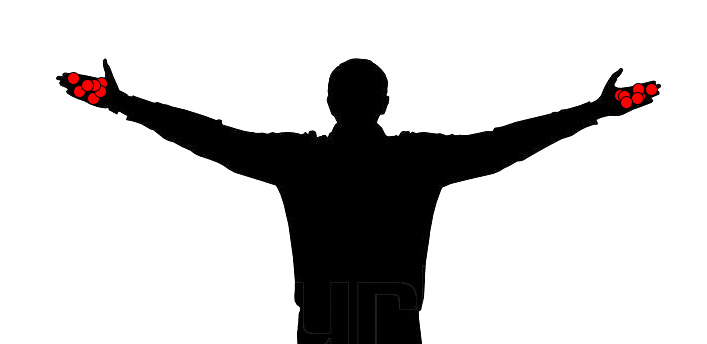
\includegraphics[width=1\linewidth]{Pictures/systemAccuratePrecise}
		\subcaption{Accurate and precise system generates measurements that are close to the real world}
		\label{fig:systemAccuratePrecise}
	\end{minipage}
	\hfill
	\begin{minipage}[t]{0.49\linewidth}
		\centering
		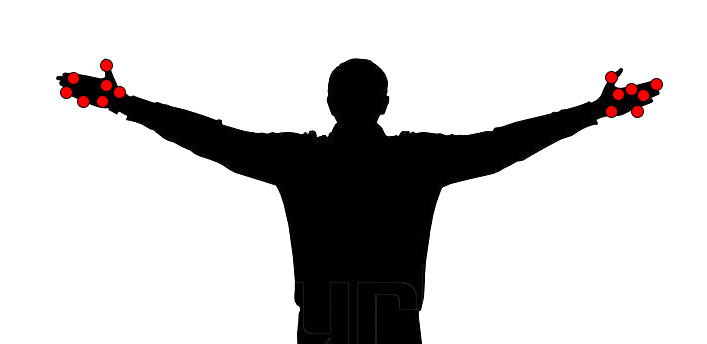
\includegraphics[width=1\linewidth]{Pictures/systemAccurateImprecise}
		\subcaption{Accurate and suffice precise system generates measurements that are close to each other and are not systematically biased}
		\label{fig:systemAccurateImprecise}
	\end{minipage}
	\caption{Definition of accuracy and precision~\cite{Woolford2015-ub}}
	\label{fig:systemAccuracyAndPrecisiong}
\end{figure}

The Microsoft Kinect v2 can indeed be compared with high performance tracking devices. If no detailed analysis is needed, it provides reliable and appropriate data. For the assistance system it should provide sufficient data to track the user and give useful feedback

\subsection{Implementation in Balance Training Scenarios}

Like already stated Chang et al.~\cite{Chang2012-hz} not only assessed the accuracy of the Microsoft Kinect but also if it could fit as an alternative training device in rehabilitation training. The results show that it provides enough usable feedback to the therapists to be an appropriate device for medical uses. Woolford~\cite{Woolford2015-ub} state that the Microsoft kinect is a useful device for monitoring such exercises. The setup is relatively easy and the tracking is appropriate for exercises in a healthcare environment. Lim et al.~\cite{Lim2015-pw} investigated the usage of Microsoft Kinect in the field of falling risk. They tracked characterizing movements and found that it is an useful device for balance training. Ustinova et al.~\cite{Ustinova2014-ml} used the Kinect to improve the postural control as well as coordination deficits from chronic traumatic brain injury patients. It resulted in improvements of postural stability, movement performance and motoric coordination. The participants were also very satisfied whereas normal exercises have been stated as boring. Pisan et al.~\cite{Pisan2013-sf} used the device to investigate the prediction of the loss of balance for elderly users with a step training program. The user preferred doing exercises with the system and the tests matched also the expectation of the researcher. An integration in promoting the postural control for parkinson disease with 

Kinect games were elaborated by Pompeu et al.~\cite{Pompeu2014-yl, Pompeu2015-vp}. The results affirm that the patients improve in balance purposes and motoric movements with this help.

Furthermore Estapa et al.~\cite{Estepa2016-oj} and Freitas et al.~\cite{Freitas2012-ae} collected data of execution from patients for medical reviews. Both developed a motor rehabilitation game. It is used to support therapeutic exercises and evaluate biomechanics of the patients. This allows subsequent analysis of the performance data for the therapist.

This approach of data analysis was also integrated by Garrido et al.~\cite{Garrido2013-zs} but in addition they elaborate if the Kinect can serve as a rehabilitation home assistance. Many patients are thrown out of their daily life environment for accessing traditional rehabilitation training in a medical center. The patient incorporate the system into their daily life and avoid such trips. The medical stuff gets all relevant parameters due to the transmission of the recordings from the exercises to the medical center. Beside this they get more time because nobody has to observe the training.

Keeping the stated results in mind shows that the Microsoft Kinect is a promising system for balance exercises that provides sufficient accurate and usable feedback. It can be embedded in a variation of fields as rehabilitation system, home assistance, or preventative technique. The aspect to motivate patients with an exergame approach and enjoyable user interface can also lead to successful exercise execution, which is part of the next section.\label{2_2_interactiveTechnology}

\section{Feedback and Interaction Methods}\label{2_4_methods}

Cognitive load plays an important role if skill acquisition is a major factor. In slacklining the user has to focus on multiple things simultaneously that increases the mental pressure. Several studies show why and how the cognitive load should be restricted. Another important fact is that repetitive exercises can lead to a boring and demotivating user experience. For that reason several methods, systems and game approaches can be used as an inspiration to build a system with a motivating and joyful environment. At last the integration and visualisation of feedback and interaction methods should be well thought out. Various techniques have been elaborated on how to provide this appropriately.

\subsection{Restricting Cognitive Load}

As a baseline Paas et al.~\cite{Paas2003-xt} describes that the acquisition of new skills is in conjunction with cognitive load. By adjusting this the learning effect can be easened or hardened. Three types of cognitive loads exists that handle the working memory of a person regarding the learning process. Intrinsic load is the inherent complexity that is caused by the topic itself. It is also important in which manner information is given to the user. If this is unnecessary, repetitive, or interferes her it is called an extraneous cognitive load and increases the burden of the user. The last type is germane cognitive load, which describes also how information is given to the user but by supporting the him in that way. This is brought by activating and automating already existing patterns or generating new ones in the working memory to enhance a learning process. Regarding this several applications have been evaluated that are also relevant to the slacklining supporting system.

Van der Spek~\cite{Van_der_Spek2010-fe} evaluated how to deal with the right complexity in serious games. He describes in his mental model construction (Figure \ref{fig:mentalModelConstruction}) that interference can be avoided by information regulation and focus attention. Improving is encouraged by predictability and reflection of the tasks. The attention of the user should be focused to relevant material by regulating the information given to him. Since a serious game like approach should be developed this is an important reference for building an effective learning process to the user.
\begin{figure}[htb]
	\centering
	\begin{minipage}[t]{1\linewidth}
		\centering
		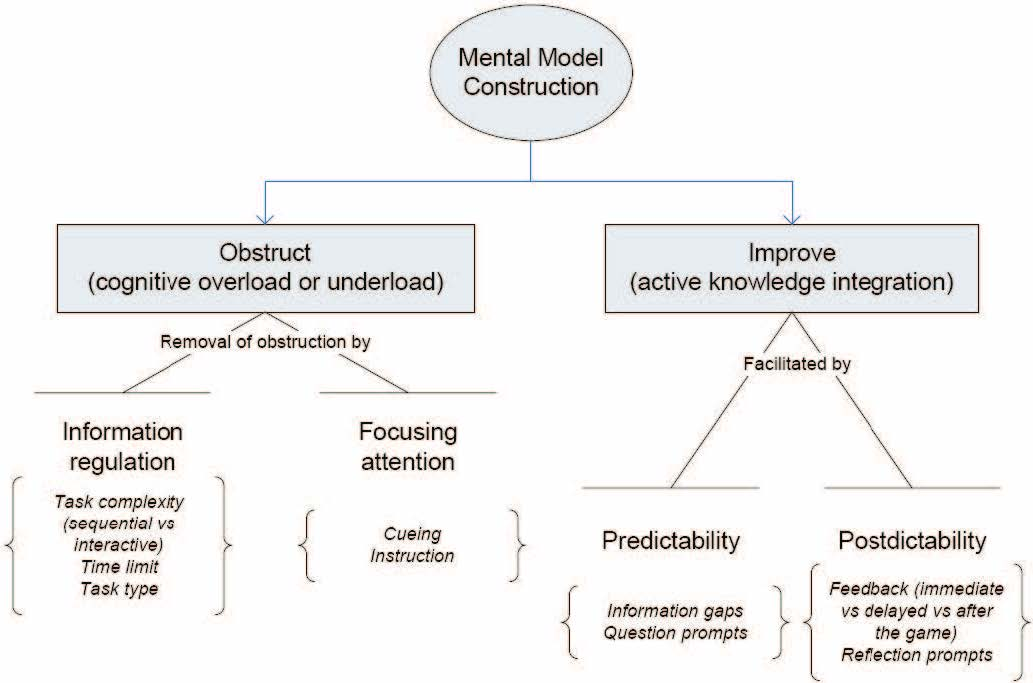
\includegraphics[width=0.74\linewidth]{Pictures/mentalModelConstruction}
		\caption{Guideline for enhancing the cognitive load~\cite{Van_der_Spek2010-fe}}
		\label{fig:mentalModelConstruction}
	\end{minipage}
\end{figure}

Pisan et al.~\cite{Pisan2013-sf} evaluates the user risk of falling with cognitive loading exercises. They executed two stroop tests, where the participant had to name the correct color of the word. High and low cognitive load can be measured by differentiating the meaning and color of a word. In the next challenge she has to answer different maths problems provided by the system. The results show that the reaction time due to cognitive load is much larger with users that have a higher risk of falling than for users that have a lower risk. This could be explainable due to the fact that user with higher falling risk are not that good in terms of switching the cognitive focus from the balancing action into other actions. 

Training on a slackline provides cognitive load to the user because of several simultaneously things she has to be aware of. Hence feedback given on how to behave in a situation should be provided in an appropriate manner to support the slacker. The system has to be aware of this and restrict the cognitive capability in the right way. Next to cognitive load the system has to ensure that the user stays motivated for the training, which is part of the following subsection.

\subsection{Motivating Factors for Skill Acquisition}

Several rehabilitation and sport training programs can be elaborated for motivating factors because the skill acquisition in slacklining resembles with them. The training procedure is a process of repetitive exercise execution. For mastering new skills and extend himself the user must have the willingness and commitment for practicing, which can be described as motivation. The self-determination theory by Ryan et al.~\cite{Ryan2000-jn, Ryan2000-gi} describes several types of motivational factors. First the intrinsic motivation, which is caused by interest to an action and satisfies the own psychological needs for self-determined behaviour. This is the fundamental stimulus for high valuable learning and practicing. Second the extrinsic motivation that is performing an activity because of an external output. The user can hereby feel externally propelled due to compliance with external regulations or she can be self-endorsed due to willingness and acceptance by the value of the practice. 

Johnson et al.~\cite{Johnson1998-hb} stated regarding rehabilitation training that if exercises and the user himself provide negative factors like boredom, repetition or long execution time it results in a discouragement. Enhancing the interaction with this trainings can lead to effective training. 
Pisan et al.~\cite{Pisan2013-sf} says that video games can help to motivate the patients through their physical training. The participants in his user tests found the games that he developed engaging. They preferred doing the exercises with the system.

Several researchers involved the motivational aspect of video games in their system. Ustinova et al.~\cite{Ustinova2014-ml} developed four custom virtual video games to elaborate the efficacy for postural deficits. First a virtual teacher where the subject has to copy its movements strictly. Second a virtual challenger that is divided into a skateboard, courtyard and an octopus game with specific exercises in which the movements of the user are more flexible. Successfully completed performance will be rewarded with a number of points. Overall the user were strongly satisfied with the gaming part of the therapy and moderate with the virtual teacher part.

Freitas et al.~\cite{Freitas2012-ae} focused on user centred development of a physiotherapeutic game that supports motor rehabilitation exercises. A plane represented the user and she has to fly through rings in the air and avoid obstacles. The patients were strongly satisfied with the game. An important factor here is the good user interface that affects the user motivation, visually presented scenario and playing technique in a positive way.

Estepa et al.~\cite{Estepa2016-oj} evaluates three developed exergames involving different psychophysical rehabilitation exercises. A virtual avatar represents the patient and orders are giving via an auditive or visual stimuli. The first two games are a series of oncoming balls placed at desired angles that the patient has to avoid with her trunk or, in the second game, with her feet. In the third exercise she has to step forward to a colored line between starting and goal position. All games were easy to understand and provide necessary feedback. The patients had a considerable interest to use the system.

Kajastila and Hämäläinen~\cite{Kajastila2014-ug} encourages monotonous parts of climbing training by adding goals and supporting the social collaboration of the participants. Hence they are making it overall more enjoyable. Six prototypes were developed. Prototypes that rely more on a training part are an easy route builder, automatic route generator and instant video feedback. For the user those were the most useful ones. The exercises that consists of a more playful part, such as a chasing animated saw that the climber has to avoid, shifted the focus away from the training part. 

With this in mind a useful training device should be considered that includes an enjoyable virtual environment. A good balance between these both is the key for successful and motivating skill acquisition. Another part of the system should also provide useful feedback to the slacker. What methods can be used for this will be discussed in the following.

\subsection{Approaches and Techniques for providing Feedback}\label{2_3_3_feedbackApproachesTechniques}

Several technological advances like video feedback, virtual environments, and auditive information can be applied for providing feedback in sport activities. Liebermann et al.~\cite{Liebermann2002-zr} evaluated those regarding their field of application. With video information costs are relatively low, it is easy accessible, and portable. It can be repetitively replayed in real-time or superposition of two video. Training in 3D virtual environments can help to improve or to familiarize with a real world skill acquisition. The user can pre-practice a skill in simulated unknown conditions like pilots in a simulated airplane. Providing appropriate auditive information can also have a relatively high impact on performance enhancement. Also the Microsoft HCI-Guidelines state that implementing audio is a good way if the user need to be notified, and to indicate states of changing behaviour~\cite{MicrosoftHIG2014-mh}. For example in balance training a warning signal can indicate that the current pose is not the desired one. If the user corrects his posture in the right way, the signal should then transform into an more comfortable signal. All of these allow qualitative and meaningful feedback in their application context. The user can review the execution, pre practice in a virtual environment, or be supported by audio warning signals. With this she can discover failure in her performance.

Feedback has to be provided in an appropriate manner for improving new motor skill acquisition. Especially for starting to learn a new technique it is important to have immediate feedback sources on which the user can rely on~\cite{Hodges2002-gb, Winstein1990-to}. Therefore it should be easy to understand for enhancing the learning process. 

Hämäläinen~\cite{Hmlinen2004-ai} developed applications for a camera output in front of the user. An automated motion controlled approach starts and stops the recording if the motion exceeds a certain threshold. Second a speech and last a gesture control prototype. Both consists of four commands to record, play, stop and delay the recording. The user test ranked the automation the worst because it reacted to unintentional motions, which ends in unwanted command recognition. The speech system ranked the best but only worked well if the participant speaks near the microphone. Some mentioned that the gesture approach were more intuitive and natural, which could be a good compromise out of the three approaches.

Holsti et al.~\cite{Holsti2013-kn} investigated delayed video feedback and a platform jumping game in trampoline sport. The former records the performance execution and shows it repetitive to the user. In the second the player has to jump back- and forwards on virtual platforms. They tested it with athletes and beginner. The delayed video feedback was ranked useful for nearly all athletes. Overall the platform jumping game was ranked the best.

Kajastila and Hämäläinen~\cite{Kajastila2014-ug} project graphics on an artificial climbing wall. A feasibility study showed that graphic information is best located near holds where the focus of the climber goes naturally. 
This can be adapted to slacklining since the slacker has to focus usually a specific point in front of her. It would be useful to provide information in the peripheral view. Next to other prototypes he has implemented an instant delayed video feedback. This is rated as one of the most useful ones because the user can immediately analyse her performance. Also a gaming approach is developed as an animated saw that chases the climber and has to be avoided. User state that it moves the focus away from the training, but it could be an enjoyable alternative to kids for getting them used to the sport. 

Based on the results of the last paper Kajastila et al.~\cite{Kajastila2016-ot} developed two games and a route creation application. User emphasize the versatility and excitement of the games. They also forget the fear of heights due to time limits and forcing them to focus and achieve a goal. User stated that playing and spectating is also more fun due to implemented sound and visual effects.

Like seen a delayed video feedback is a good approach to learn new skills. Combining this with a gaming approach can simultaneously lead to a joyful experience with training aspects. Also adding audio signals can further improve this experience for the user as well as for spectators. A well suited interaction mechanism and a good looking environment can help to create an effective system and motivate the user for training purposes.

%Kann evtl nicht genutzt werden
%Displaying an avatar can be further implemented by a conjunction or overlapping with an instructor on the screen \textbf{(Figure 8)}. With this she can see wrong performance execution in real time. After the exercise she should be able to review her performance. At the same time the system has to be aware of not distracting the user too much during the performance. \label{2_3_feedbackMethods}

\section{User Interface Design}
The user interacts with the system through the provided interface. This should contain all relevant information, which are necessary to achieve a specific goal and support her on the way to reach this goal. General user interface approaches from exergame like related work approaches should be compared. Therefore the subsection \textit{\nameref{2_5_1_userInterfacefeedback}} gives an overview on which elements can be used for guiding the user through the system and how feedback can be visualized properly. After that in subsection \textit{\nameref{2_5_2_kinectHIG}} shows how to enhance the user experience on a kinect application with guidelines provided by Microsoft.

\subsection{User interface design for appropriate feedback}\label{2_5_1_userInterfacefeedback}

Important feedback information during the exercise should be placed surrounding the focus point in the peripheral view of the user. Directing the user for correcting her movement can be done in several ways. Basic information about the execution should be given prior to the user for exercise preparation. Surrounding objects can be displayed as arrows, flashing notifications or weighting scale like seen by Garrido et al.~\cite{Garrido2013-zs} in Figure \ref{fig:informationUISurroundingObjects}. 
\begin{figure}[htb]
	\centering
	\begin{minipage}[t]{0.49\linewidth}
		\centering
		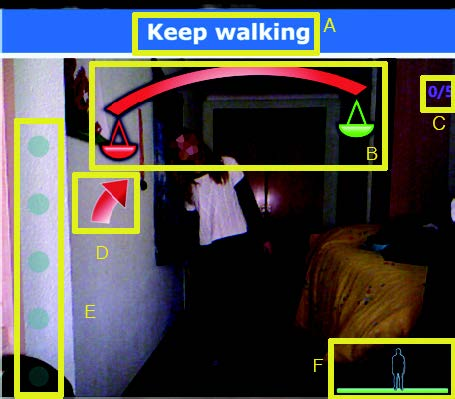
\includegraphics[width=1\linewidth]{Pictures/informationUISurroundingObjects}
		\subcaption{Surrounding elements in the interface}
		\label{fig:informationUISurroundingObjects}
	\end{minipage}
	\hfill
	\begin{minipage}[t]{0.49\linewidth}
		\centering
		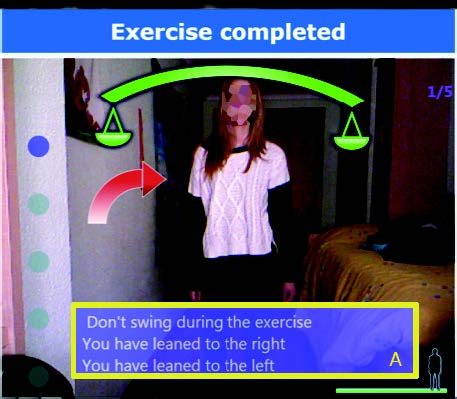
\includegraphics[width=1\linewidth]{Pictures/informationUIFeedbackSummary}
		\subcaption{Completed exercise feedback summary}
		\label{fig:informationUIFeedbackSummary}
	\end{minipage}
	\caption{Interface of a rehabilitation training application~\cite{Garrido2013-zs}}
	\label{fig:informationUIGarrido}
\end{figure}
Additional informations like the current exercise and the state can be displayed outside of the focus space. They should be designed to not distract the user. A feedback summary after the execution can give an useful recap about the exercise for reflection (Figure \ref{fig:informationUIFeedbackSummary}).

Another method is to show the user itself or an avatar that demonstrates the correct performance of the current exercises like in Figure \ref{fig:avatar3DModel} and \ref{fig:avatarUser}. Holsti et al.~\cite{Holsti2013-kn} implemented such a user integration and in user testing they endorse to see themself performing in real time.
\begin{figure}[htb]
	\centering
	\begin{minipage}[t]{0.49\linewidth}
		\centering
		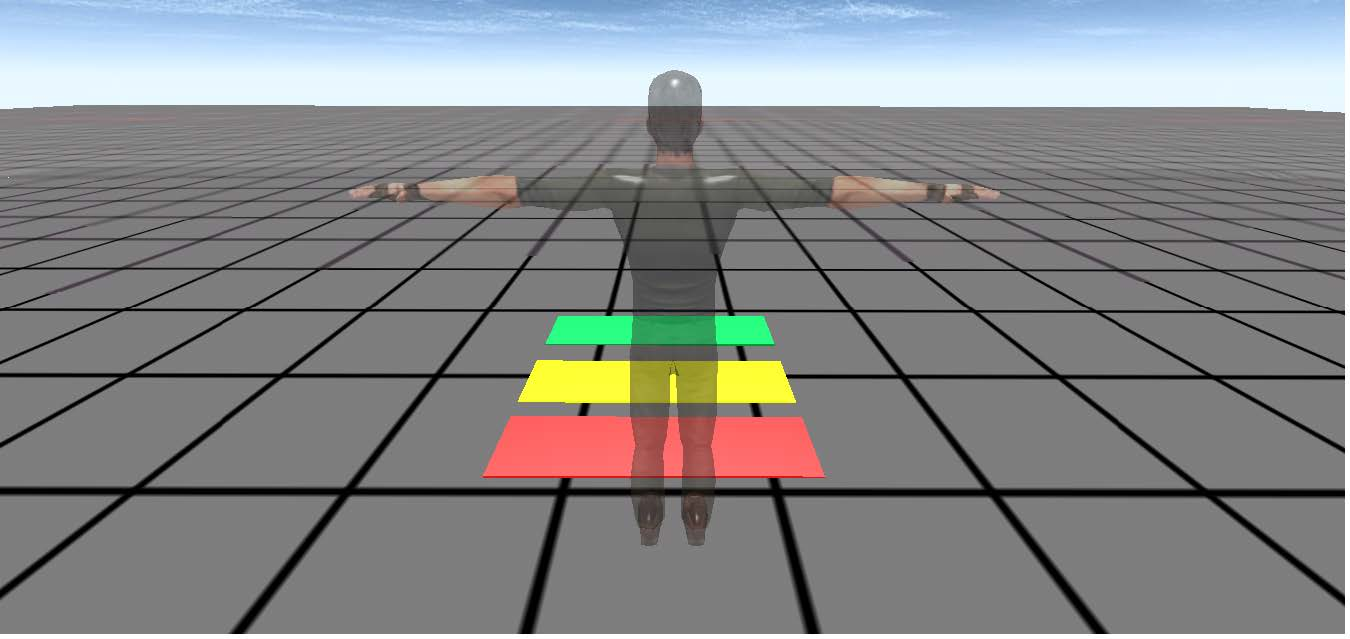
\includegraphics[width=1\linewidth]{Pictures/avatar3DModel}
		\caption{3D Model as avatar~\cite{Estepa2016-oj}}
		\label{fig:avatar3DModel}
	\end{minipage}
	\hfill
	\begin{minipage}[t]{0.49\linewidth}
		\centering
		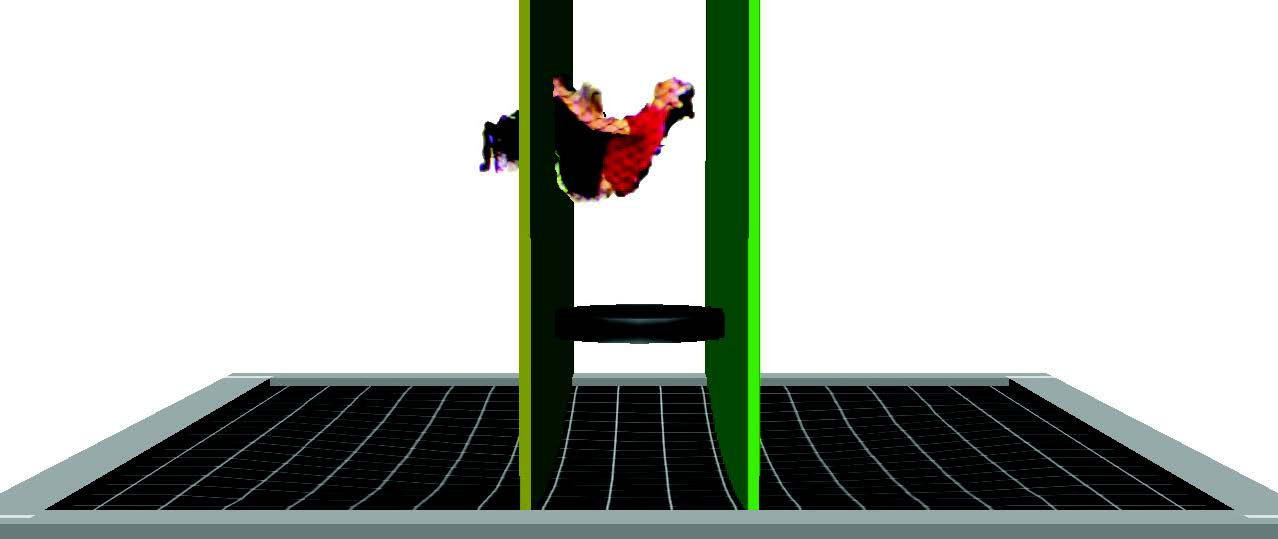
\includegraphics[width=1\linewidth]{Pictures/avatarUser}
		\caption{Rail-time user representation~\cite{Holsti2013-kn}}
		\label{fig:avatarUser}
	\end{minipage}
\end{figure}

The task about the execution has to be clarified. Chang et al.~\cite{Chang2012-hz} provides real time feedback on the performance quality due to a visualised path. If the performance is correct the path will turn green. But if she moves outside the range the path turns red and an arrows guides him into the correct position. Instructions and highlighting objects can help to complete an exercise successfully (Figure \ref{fig:gameUIChang}). If she performs something wrong during the performance e.g. in the slacklining case corresponding body parts could be highlighted.
\begin{figure}[htb]
	\centering
	\begin{minipage}[t]{0.49\linewidth}
		\centering
		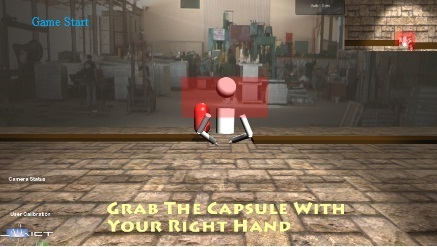
\includegraphics[width=1\linewidth]{Pictures/gameInstruction}
		\subcaption{Instruction to the game}
		\label{fig:gameInstruction}
	\end{minipage}
	\hfill
	\begin{minipage}[t]{0.49\linewidth}
		\centering
		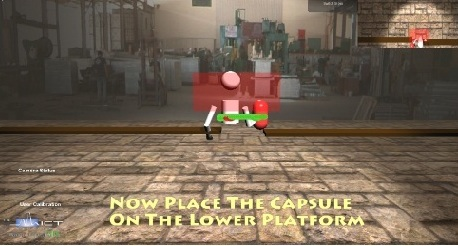
\includegraphics[width=1\linewidth]{Pictures/gameHighlighting}
		\subcaption{Green indicator for correct performance}
		\label{fig:gameHighlighting}
	\end{minipage}
	\caption{User interface of a rehabilitational application~\cite{Chang2012-hz}}
	\label{fig:gameUIChang}
\end{figure}

\subsection{Kinect for Windows - Human Interface Guidelines}\label{2_5_2_kinectHIG}
Microsoft itself offers Human-Interface-Guidelines (HIG) for developer and designer that describes several techniques of certain areas for developing a kinect application~\cite{MicrosoftHIG2014-mh}. It provides a quick introduction into the Kinect itself, design principles for interactions regarding gesture and voice, techniques on teaching complex gestures, and how to visualize appropriate feedback. Also which interactions should be used for a specific action. Therefore developer may follow this general standard to support their end-user. In the following general principles of the guideline will be discussed on which the interactive slackline system will rely on to enhance the user experience. 
%The general design principles are that the application should be context-aware, make the user confident, choosing the right input method and to conduct user tests. 

\subsubsection{Basic design principles}
Context-awareness delivers the best user experience e.g. controls should be placed where user would expect them to be and interactions should be appropriate for the environment. It is important that the user feel confident by designing interactions simple and easy to learn. User will choose an input that take the least effort for the given goal. Therefore the input method should match its purpose, be reliable, consistent, and convenient. Conducting user test helps to improve the system. Not each person will use the system the same way and minor adjustments can make a huge difference in the understanding of the usage.

\subsubsection{Visual and audio feedback}
Giving the user constant feedback helps her to know what is happening. In general appropriate feedback should show if the sensor is ready, she is visible and engaging with the Kinect, and so on (Figure \ref{fig:hciGuidelinesFeedbackCursor}). Regarding this a combination of visual as well as audio feedback results in a better experience, e.g. clicking a button changes its visual state and provides an audio signal (Figure \ref{fig:hciGuidelinesFeedbackControl}).
\begin{comment}
\begin{figure}[htb]
	\centering
	\begin{minipage}[t]{0.45\linewidth}
		\centering
		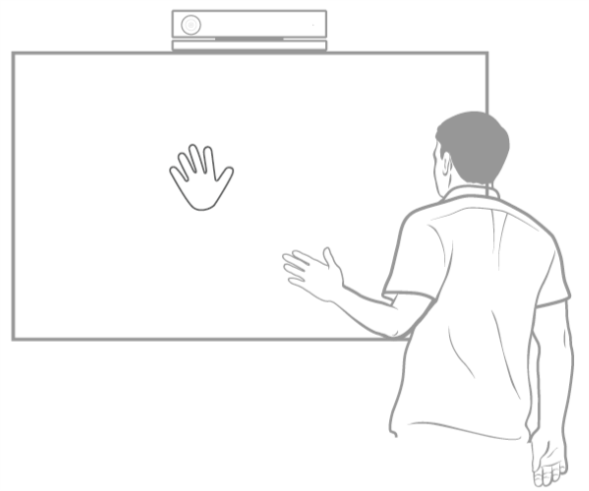
\includegraphics[width=0.5\linewidth]{Pictures/hciGuidelinesFeedbackCursor}
		\caption{Hand cursor visualizes the engagement and readiness of the system~\cite{MicrosoftHIG2014-mh}}
		\label{fig:hciGuidelinesFeedbackCursor}
	\end{minipage}
	\hfill
	\begin{minipage}[t]{0.45\linewidth}
		\centering
		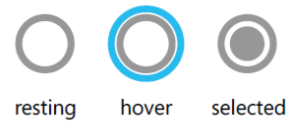
\includegraphics[width=0.5\linewidth]{Pictures/hciGuidelinesFeedbackControl}
		\caption{Different states of UI controls~\cite{MicrosoftHIG2014-mh}}
		\label{fig:hciGuidelinesFeedbackControl}
	\end{minipage}
\end{figure}
\end{comment}
\begin{figure}[htb]
	\centering
	\begin{minipage}[t]{0.45\linewidth}
		\centering
		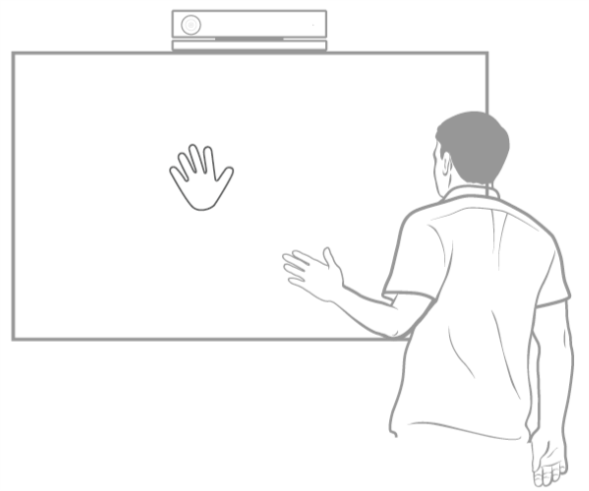
\includegraphics[width=0.5\linewidth]{Pictures/hciGuidelinesFeedbackCursor}
		\subcaption{Hand cursor visualizes the engagement and readiness of the system}
		\label{fig:hciGuidelinesFeedbackCursor}
	\end{minipage}
	\hfill
	\begin{minipage}[t]{0.45\linewidth}
		\centering
		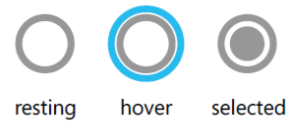
\includegraphics[width=0.5\linewidth]{Pictures/hciGuidelinesFeedbackControl}
		\subcaption{Different states of UI controls}
		\label{fig:hciGuidelinesFeedbackControl}
	\end{minipage}
	\caption{Feedback methods~\cite{MicrosoftHIG2014-mh}}
	\label{fig:hciGuidelinesFeedback}
\end{figure}

The most important part for complex gestures is the progress indicator described in this guideline. It supports the user if she has to hold a position, as well as if an amount of frequent repetitions have to be performed. Clear and prominent visuals should be used to show the entire progression (Figure \ref{fig:visualFeedbackIndicator}). If a user has to copy a specific movement an avatar or animation can be shown, before or during the movement, like in Figure \ref{fig:visualFeedbackAvatar}.
\begin{figure}[htb]
	\centering
	\begin{minipage}[t]{0.49\linewidth}
		\centering
		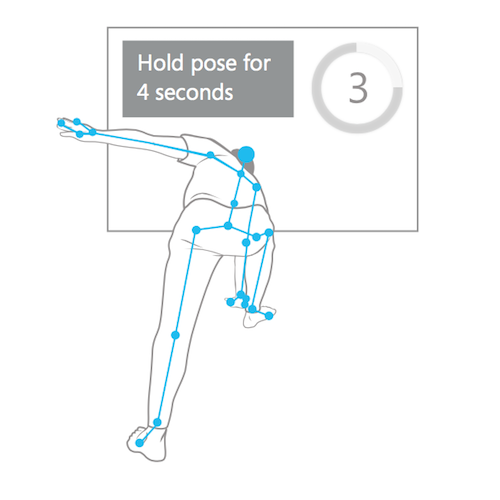
\includegraphics[width=0.9\linewidth]{Pictures/2_4_visualFeedbackIndicator}
		\subcaption{Repetition and time length indicators}
		\label{fig:visualFeedbackIndicator}
	\end{minipage}
	\hfill
	\begin{minipage}[t]{0.49\linewidth}
		\centering
		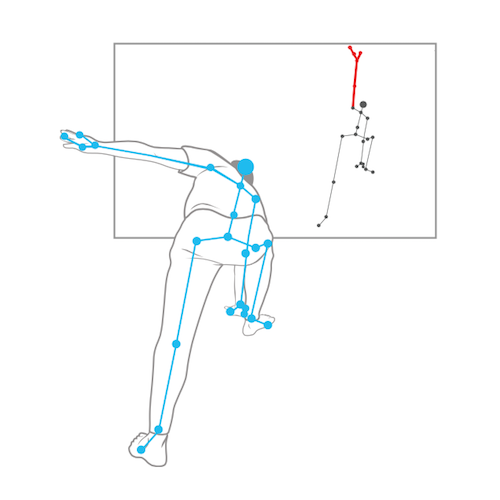
\includegraphics[width=0.9\linewidth]{Pictures/2_4_visualFeedbackAvatar}
		\subcaption{Avatar that shows correct movement and wrong body parts are highlighted}
		\label{fig:visualFeedbackAvatar}
	\end{minipage}
	\caption{Feedback indicator and movement visualization as an avatar~\cite{MicrosoftHIG2014-mh}}
	\label{fig:hciGuidelinesIndicatorAvatar}
\end{figure}

\subsubsection{Clarification}
The user may interpret interactions with the system differently from others. Therefore the system should explain clearly what the user has to do, e.g. \textit{"Raise one hand above your head"} instead of just \textit{"Raise your hand"}. The cognitive load of the user should be kept low and not exceed a number of six gestures, such that she easily remembers the actions. The system has a set of three basic interaction techniques, which fits in this range.

\subsubsection{User viewer}
A small scene viewer shows the range in which the user can move and is recognized by the Kinect. It displays a mirror like view in which the user can see a silhouette of herself and the constraints of the Kinect device, like in figure \ref{fig:higUserViewer}.
\begin{figure}[htb]
	\centering
	\begin{minipage}[t]{1\linewidth}
		\centering
		
\includegraphics[width=0.6\linewidth]{Pictures/higUserViewer}
		\caption{User Viewer on top~\cite{MicrosoftHIG2014-mh}}
		\label{fig:higUserViewer}
	\end{minipage}
\end{figure}

\subsubsection{Learning interaction methods}
The application should teach the user how to proper interact with it right from the beginning with an introduction tutorial. An interaction itself should rely on the real world, which can help the user to be more familiar with the product, than learning unknown gestures (Figure \ref{fig:hciGuidelinesDynamicGesture}). Also biliteral interaction support should be applied to cover both possibilities for left- and right-handed people.
\begin{figure}[htb]
	\centering
	\begin{minipage}[t]{1\linewidth}
		\centering
		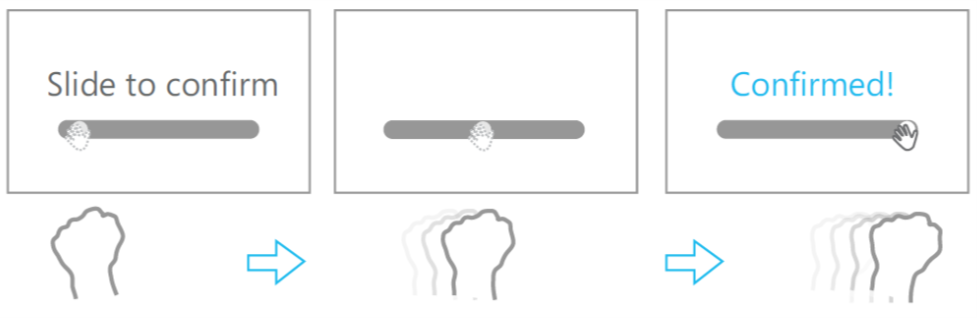
\includegraphics[width=0.6\linewidth]{Pictures/hciGuidelinesDynamicGesture}
		\caption{Direct manipulation of a slider with intuitive interaction~\cite{MicrosoftHIG2014-mh}}
		\label{fig:hciGuidelinesDynamicGesture}
	\end{minipage}
\end{figure}

\subsubsection{Teaching complex gestures / exercises}
Executing gestures is a core functionality in the slacklining assistance system. For new gestures, especially complex ones, the application should provide a tutorial that teaches and shows the user on how to execute or accomplish the gesture properly. When performing the gesture a visual indicator (a hint, animation, or notification) should acknowledge if the gesture is executed and when it is completed. (Figure \ref{fig:hciGuidelinesTeachingMethods}).
\begin{figure}[htb]
	\centering
	\begin{minipage}[t]{1\linewidth}
		\centering
		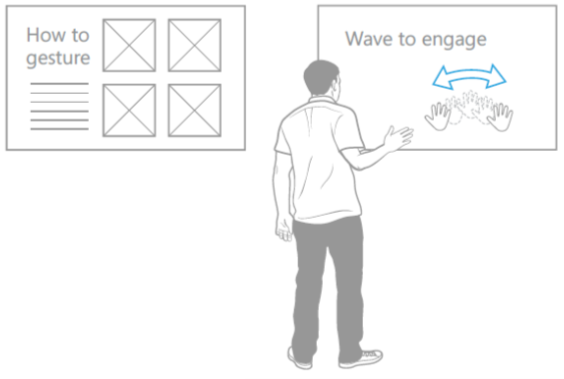
\includegraphics[width=0.4\linewidth]{Pictures/hciGuidelinesTeachingMethods}
		\caption{Teaching new gestures~\cite{MicrosoftHIG2014-mh}}
		\label{fig:hciGuidelinesTeachingMethods}
	\end{minipage}
\end{figure}

\subsubsection{Element sizing}
The system will rely on the guidelines and match the button sizing regarding the screen resolution to keep reliability on interaction. This is a size of 208 by 208px in a resolution of 1920x1080 pixel. As recommended a tile button style will be used which are a good baseline where the user can hit them accurately and read the button text.

\subsubsection{Physical interaction zone}
This zone ensures that the user is able to reach anything in a comfortable range. In the application it is constrained by the joints of the shoulders to the hips of the opposite site of the interaction hand. It is designed like seen in figure \ref{fig:higPHIZ} to have a better understanding.
\begin{figure}[htb]
	\centering
	\begin{minipage}[t]{1\linewidth}
		\centering
		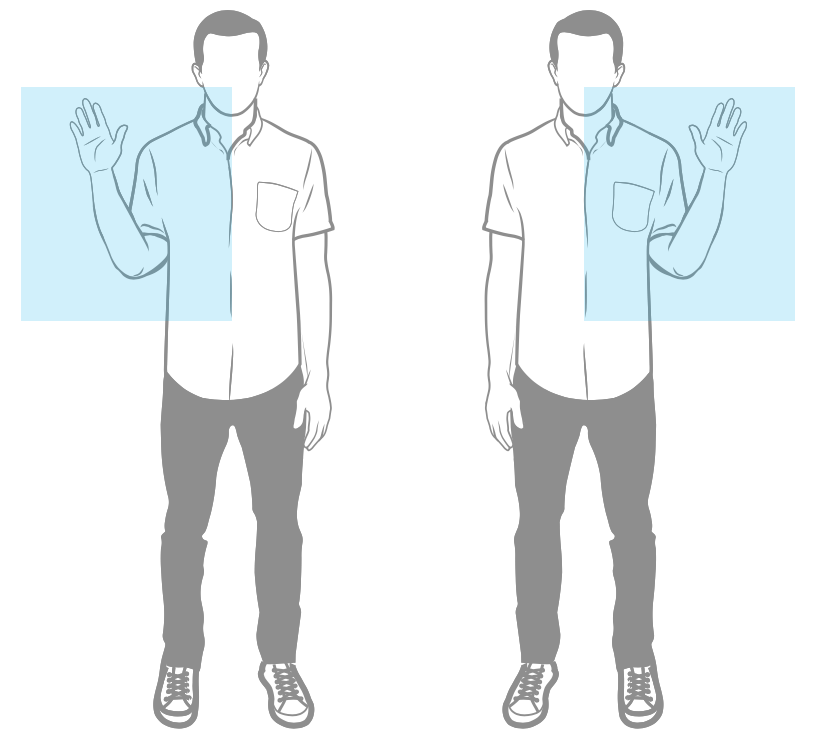
\includegraphics[width=0.32\linewidth]{Pictures/higPHIZ}
		\caption{Physical interaction zone~\cite{MicrosoftHIG2014-mh}}
		\label{fig:higPHIZ}
	\end{minipage}
\end{figure}

\begin{comment}
- System should provide a user view, such that the user knows the constraints of the kinect tracking area --> should be small if interacting in menu and big if needed in execution for example
\\- Audio feedback (success/failing)
\\- Big buttons/selectable elements
\\- Button state changes --> visualize
\\- \todo{picture of key elements from Kinect HIG}

- \todo{maybe combine interaction with key elements of a kinect application}
\end{comment}


Summarizing the user interface should not distract the slacker but support him. Only necessary and useful information have to be displayed during the exercise. Providing an introduction and useful tips can help to give an understanding of the exercise. An avatar or animation is a good alternative to make clear how to perform an exercise. The system should also rely on Microsoft human interface guidelines, which provides design tips and serves as a reference to build user friendly applications.
\label{2_4_uiDesign}

\section{Conclusion}
With the stated related work a foundation is given to build a slacklining assistance system. For teaching beginners on a slackline it is important get familiar with it. The assistance system should provide the given exercises and tips for beginners which build a foundation for further training.
%like focusing the eye and turning the hands over the shoulder, 
Several application scenarios show that slacklining can replace balance training in rehabilitation environment, as prevention system, in school sport or as an home assistance. This can be combined with interactive technology, which helps patients to fulfil their exercises and provide the medical stuff with sufficient analysis data.

As interaction device the Microsoft Kinect v2 seems like the best choice out of the available technologies. It provides sufficient useful and accurate data analysis, if no in-depth analysis is needed. More advantages are the low cost, short setup time and the freedom of the movements for the user. Several studies indicate also that the Kinect can be embedded in balance training scenarios and increases the training efficacy while motivate patients.

A problem that occurs with more complexity in the exercises is the raising cognitive load. The system should therefore provide appropriate feedback and be aware of the cognitive load of the slacker. Motivating the slacker for further exercise execution can be done with a well defined interaction mechanism, an enjoyable but challenging virtual training environment, and an user friendly interface. This can be realised especially with the help of human interface guidelines provided by Microsoft, which include several design tips for developing a Kinect application.

With the help of this foundation a concept for the slacklining assistance system has been created, which can be seen in the next chapter.
\newpage
